\newpage

\clearpage

\includegraphics[scale=0.03]{Figures/NMACN.png}\href{https://compneuro.neuromatch.io/tutorials/intro.html}{\textbf{\Huge{Neuromatch Academy: Calculus Refresher - Summary Sheet}}\footnote{’t Hart et al., (2022). Neuromatch Academy: a 3-week, online summer school in computational neuroscience. Journal of Open Source Education, 5(49), 118. https://doi.org/10.21105/jose.00118}}
\begin{multicols}{3}
\clearpage
\begin{textbox}{\href{https://compneuro.neuromatch.io/tutorials/W0D4_Calculus/student/W0D4_Tutorial1.html}{Differentiation and Integration (W0D4T1)}  }
\begin{subbox}{subbox}{Introduction}
\scriptsize
\textbf{Differentiation} of a function $f(t)$ gives you the derivative of that function \begin{equation} \frac{d(f(t))}{dt}.
\end{equation} A derivative captures how sensitive a function is to slight changes in the input for different ranges of inputs. 

\textbf{Integration} can be thought of as the reverse of differentiation
\begin{equation}
\int f(t)dt.
\end{equation}
\centering
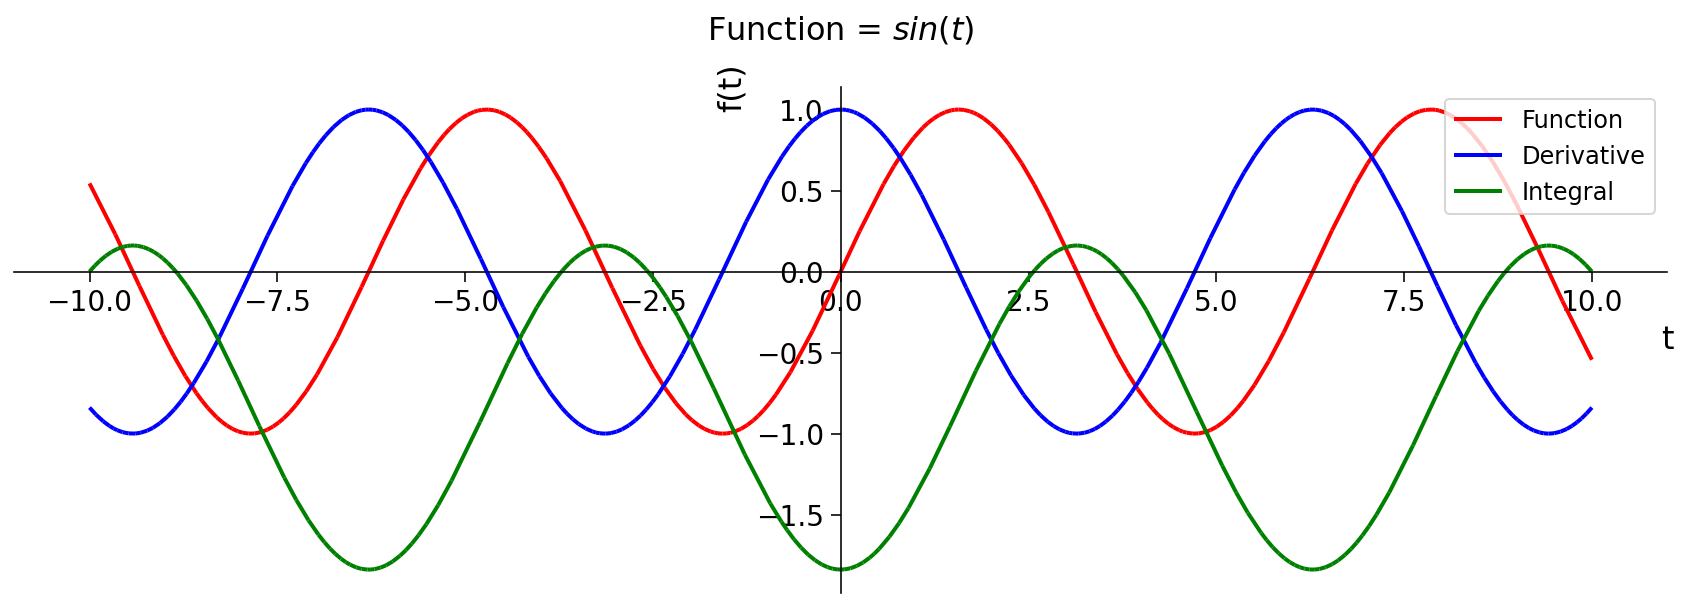
\includegraphics[scale=0.15]{Figures/PreCourse/CFigure1.png}
\end{subbox}

\begin{subbox}{subbox}{Analytical Differentiation}
\scriptsize{
When we find the derivative analytically, we are finding the exact formula for the derivative function. 
To do this, instead of having to do some fancy math every time, we can consult a list of common derivatives such as:

\textbf{ \href{https://en.wikipedia.org/wiki/Product_rule}{The Product Rule}}
\begin{align}
f(t) &= u(t)\cdot v(t) \\
\frac{d(f(t))}{dt} &= v\cdot \frac{du}{dt} + u\cdot \frac{dv}{dt}
\end{align}
\textbf{\href{https://en.wikipedia.org/wiki/Chain_rule}{The Chain Rule}:}
\begin{equation}
\frac{dr}{da} = \frac{dr}{dt}\cdot\frac{dt}{da}.
\end{equation}
}
\end{subbox}
\begin{subbox}{subbox}{Numerical Differentiation}
\scriptsize{Formally, the numerical approximation of the derivative of a function $f(x)$ at any value $a$ is given by the finite difference formula (FD): 
\begin{equation}
FD = \frac{f(a+h) - f(a)}{h}
\end{equation}
As $h\rightarrow 0$, the FD approaches the actual value of the derivative.}

\centering
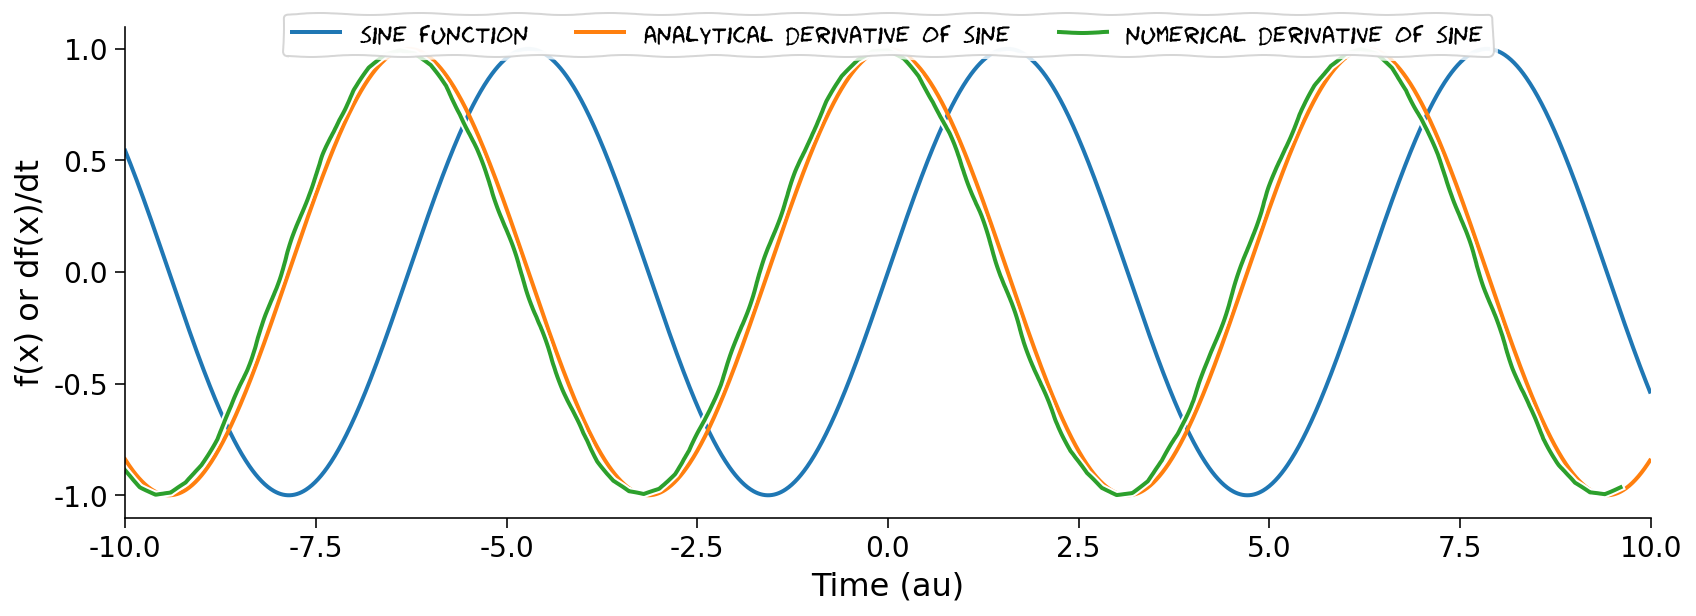
\includegraphics[scale=0.13]{Figures/PreCourse/CFigure2.png}
\end{subbox}
\end{textbox}
%%%%%%%%%%%%%%%%%%%%%%%%%%%%%%%%%%%%%%%%%%%%%%%%%%
\begin{textbox}{Differentiation and Integration (W0D4T1) }
%%%%%%%%%%%%%%%
\begin{subbox}{subbox}{Functions of Multiple Variables}
\scriptsize
In most cases, we encounter functions of multiple variables. For example, in the brain, the firing rate of a neuron is a function of both excitatory and inhibitory input rates. In the following, we will look into how to calculate derivatives of such functions.

When we take the derivative of a multivariable function with respect to one of the variables it is called the **partial derivative**. For example if we have a function:

\begin{align}
f(x,y) = x^3  +2xy+ y^2
\end{align}

The we can define the partial derivatives as

\begin{align}
\frac{\partial(f(x,y))}{\partial x} = 3x^2  +2y+ 0 \\
\frac{\partial(f(x,y))}{\partial y} = 0+ 2x+2y
\end{align}
\centering
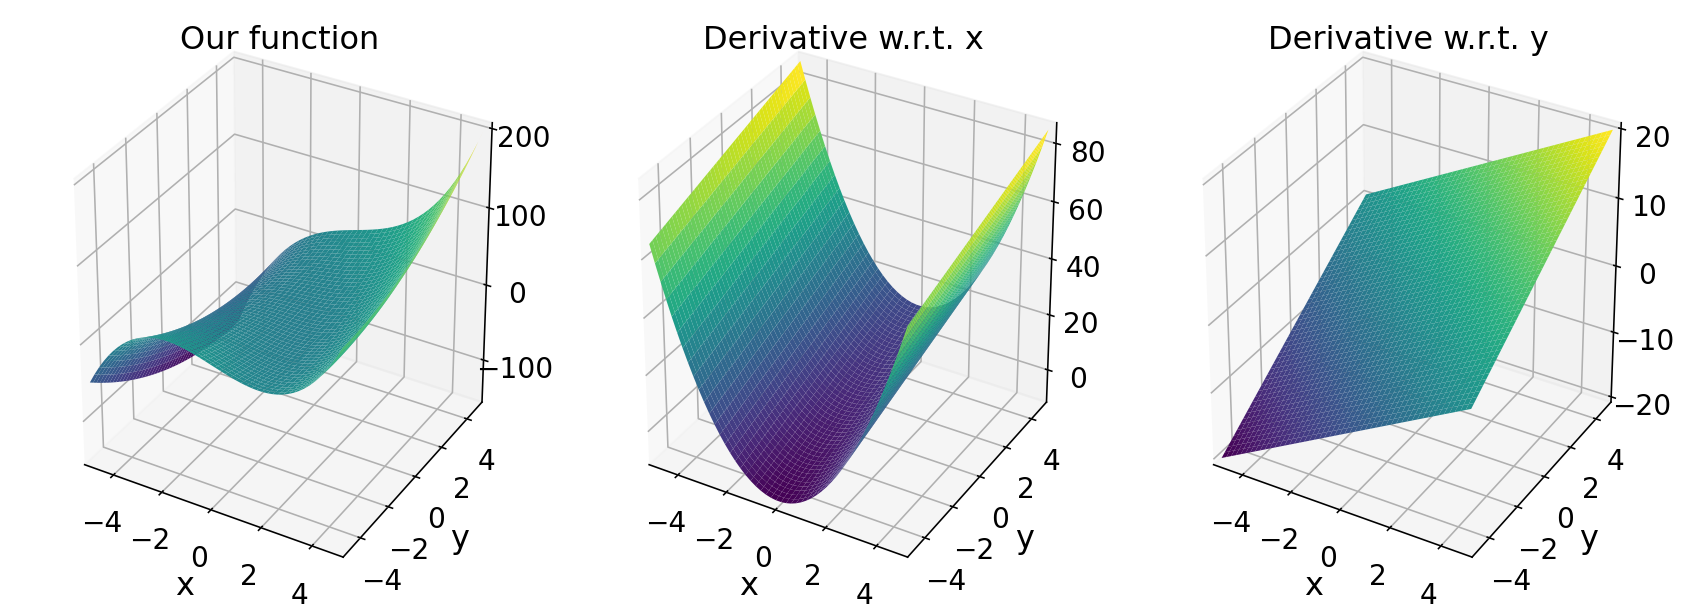
\includegraphics[scale=0.2]{Figures/PreCourse/CFigure3.png}

\end{subbox}
\begin{subbox}{subbox}{Numerical Integration (Riemann Sum)}
\scriptsize

Geometrically, integration is the area under the curve. This interpretation gives two formal ways to calculate the integral of a function numerically. 

If we wish to integrate a function $f(t)$ with respect to $t$, then first we divide the function into $n$ intervals of size $dt = a-b$, where $a$ is the starting of the interval. Thus, each interval gives a rectangle with height $f(a)$ and width $dt$. By summing the area of all the rectangles, we can approximate the area under the curve. As the size $dt$ approaches to zero, our estimate of the integral approaches the analytical calculation. 

\centering
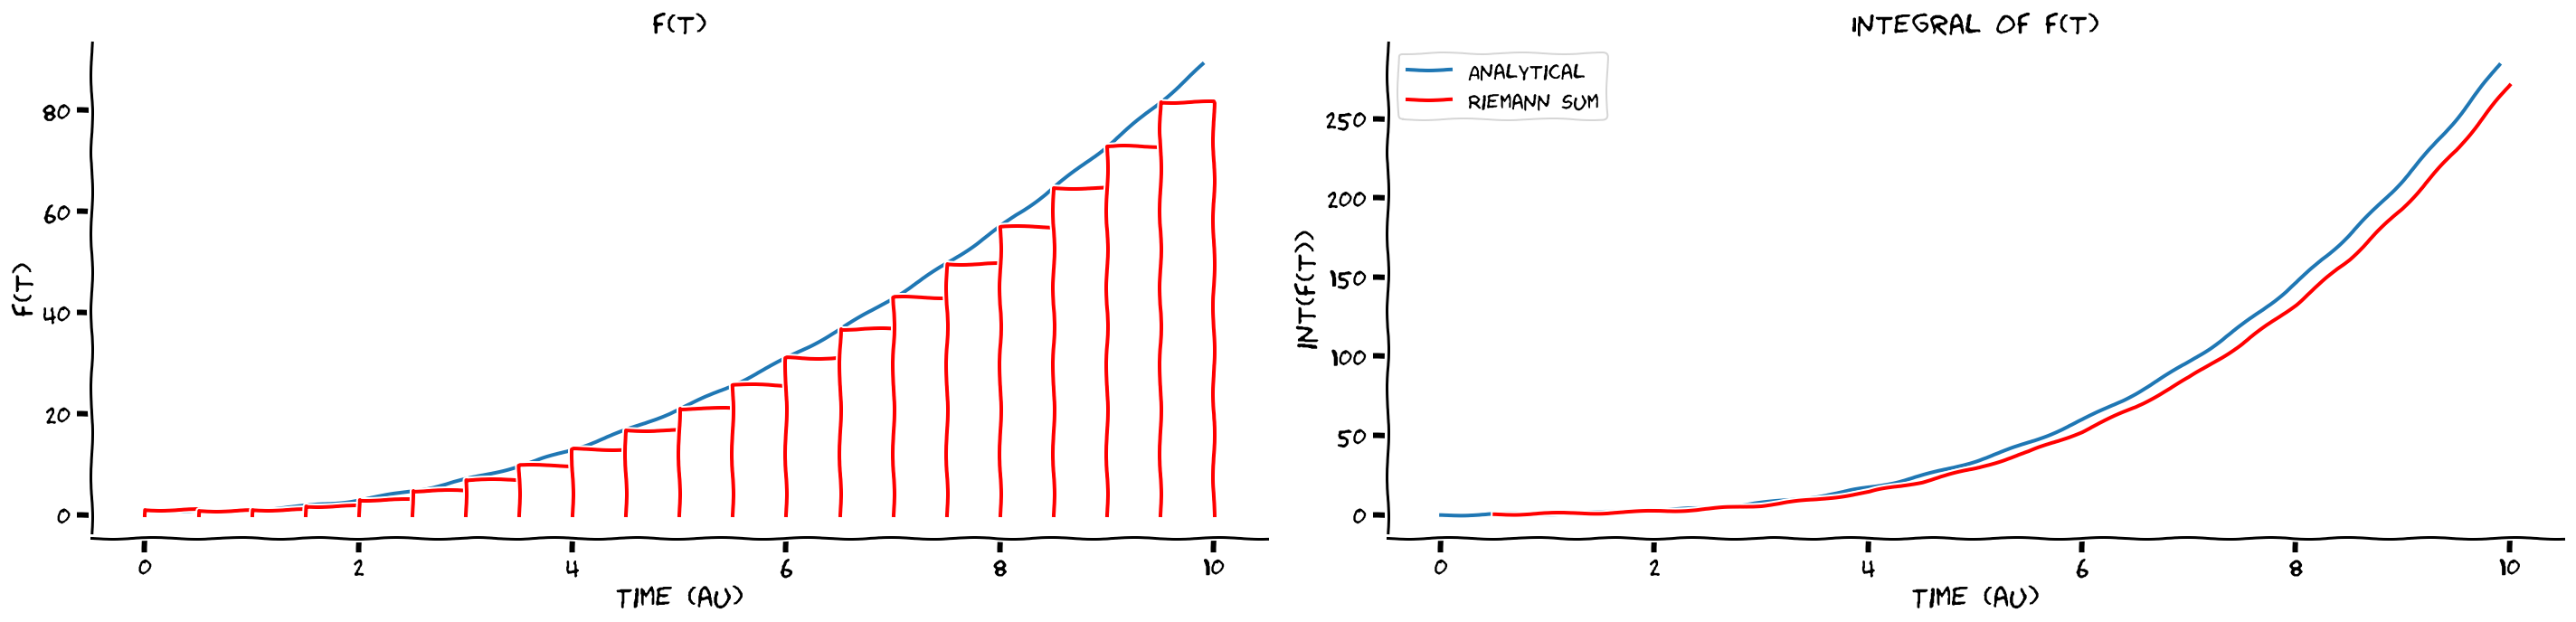
\includegraphics[scale=0.12]{Figures/PreCourse/CFigure4.png}
\end{subbox}


\end{textbox}
%%%%%%%%%%%%%%%%%%%%%%%%%%%%%%%%%%%%%%%%%%%%%%%%%%
%%%%%%%%%%%%%%%%%%%%%%%%%%%%%%%%%%%%%%%%%%%%%%%%%%
\begin{textbox}{Differential Equations (W0D4T2) }
%%%%%%%%%%%%%%%
\begin{subbox}{subbox}{Introduction}
\scriptsize
Differential Equations are mathematical equations that describe how to solve something like population or a neuron changes over time. The reason why differential equations are so useful is they can generalise a process such that one equation can be used to describe many different outcomes.
The general form of a first order differential equation is:

\begin{equation}
\frac{d}{dt}y(t) = f\left( t,y(t) \right)
\end{equation}

which can be read as "the change in a process $y$ over time $t$ is a function $f$ of time $t$ and itself $y$".

\end{subbox}
\begin{subbox}{subbox}{Population Differential Equation}
\scriptsize
The linear population equation 
\begin{equation}
\frac{d}{dt}p(t) = \alpha p(t), \, p(0)=P_0
\end{equation}

has the exact solution:$p(t) = P_0 e^{\alpha t}.$
The exact solution written in words is: 
%\begin{equation*}
\begin{align*}
\text{"Population"} &= \text{"grows/declines exponentially as}\\ &\text{ a function of time and birth rate"}.
\end{align*}
\centering
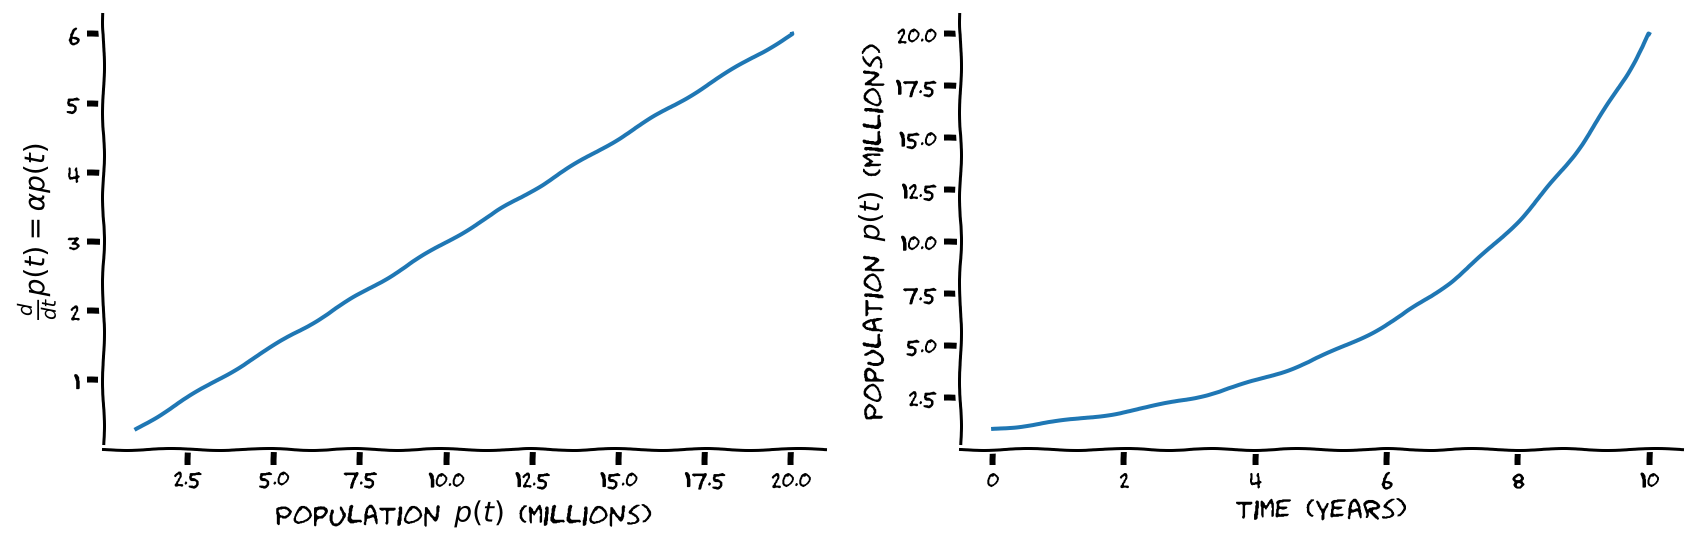
\includegraphics[scale=0.13]{Figures/PreCourse/CFigure5.png}
\end{subbox}
\begin{subbox}{subbox}{The leaky integrate and fire (LIF) model}
\scriptsize
The Leaky Integrate and Fire Model is a linear differential equation that describes the membrane potential ($V$) of a single neuron which was proposed by Louis Édouard Lapicque in 1907.

The subthreshold membrane potential dynamics of a LIF neuron is described by
\begin{align}
\tau_m\frac{dV}{dt} = -(V-E_L) + R_mI\,
\end{align}
where $\tau_m$ is the time constant, $V$ is the membrane potential,  $E_L$ is the resting potential, $R_m$ is membrane resistance, and $I$ is the external input current. 

\centering
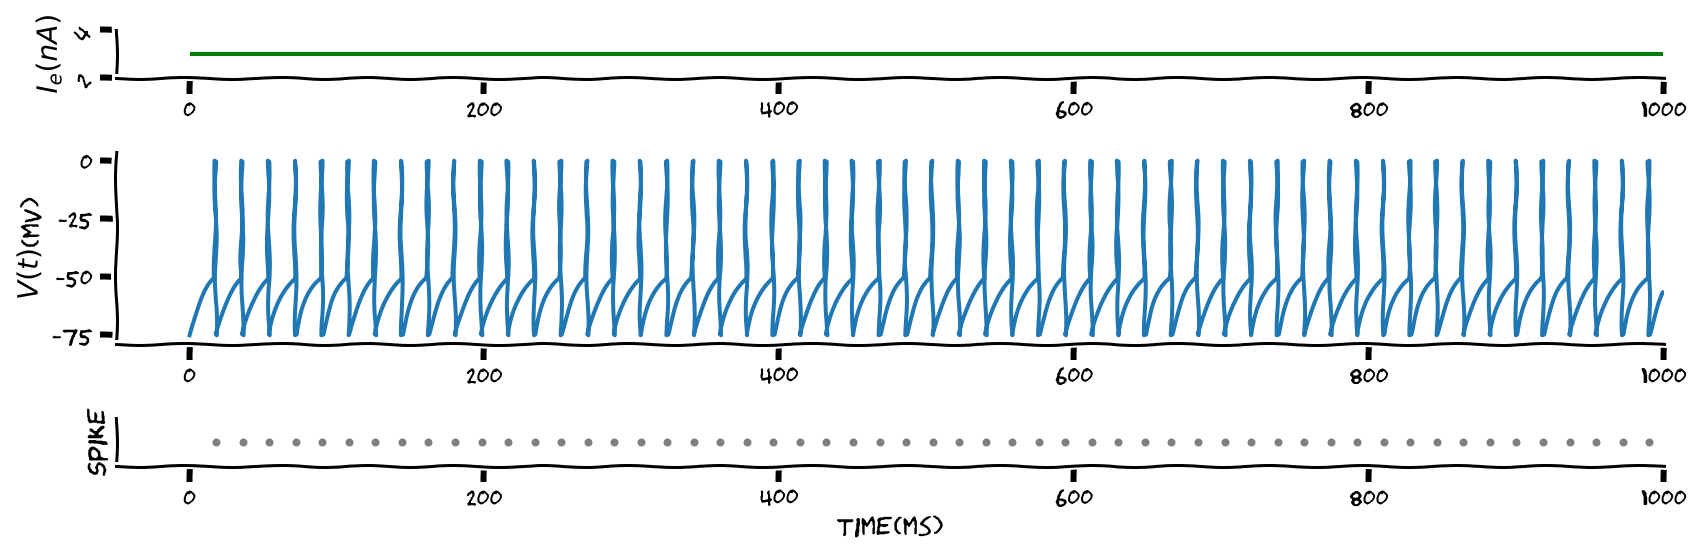
\includegraphics[scale=0.15]{Figures/PreCourse/CFigure6.png}
\end{subbox}
\end{textbox}
%%%%%%%%%%%%%%%%%%%%%%%%%%%%%%%%%%%%%%%%%%%%%%%%%%
%%%%%%%%%%%%%%%%%%%%%%%%%%%%%%%%%%%%%%%%%%%%%%%%%%
%%%%%%%%%%%%%%%%%%%%%%%%%%%%%%%%%%%%%%%%%%%%%%%%%%
\begin{textbox}{Numerical Methods (W0D4T3) }
%%%%%%%%%%%%%%%
\begin{subbox}{subbox}{Euler Method}
\scriptsize
The Euler method is one of the straight forward and elegant methods to approximate a differential. It was designed by \href{https://en.wikipedia.org/wiki/Leonhard_Euler}{Leonhard Euler (1707-1783).} 
Simply put we just replace the derivative in the differential equation by the formula for a line and re-arrange.

The slope is the rate of change between two points. The formula for the slope of a line between the points $(t_0,y(t_0))$ and $(t_1,y(t_1))$ is given by:
$$ m=\frac{y(t_1)-y(t_0)}{t_1-t_0}=\frac{\Delta y_0}{\Delta t_0}, $$
where $\Delta y_0=y_1-y_0$ and $\Delta t_0=t_1-t_0$ or in words as
$$ m=\frac{\text{ Change in y} }{\text{Change in t}}. $$
The slope can be used as an approximation of the derivative such that
$$ \frac{d}{dt}y(t)\approx \frac{y(t_0+\Delta t)-y(t_0)}{t_0+\Delta t-t_0}=\frac{y(t_0+dt)-y(t_0)}{\Delta t}$$
where $\Delta t$ is a time-step.
\end{subbox}
\begin{subbox}{subbox}{Population Differential Equation}
\scriptsize
To numerically estimate the population differential equation we replace the derivative with the slope of the line to get the discrete (not continuous) equation where $p_1$ is the estimate of $p(t_1)$. Let $\Delta t=t_1-t_0$ be the time-step and re-arrange the equation gives
\begin{align*}
\color{red}{p_1}&=\color{green}{p_0}+\color{blue}{\Delta t} (\color{blue}{\alpha} \color{green}{p_0} \color{blue}{)}
\end{align*}

where $\color{red}{p_1}$ is the unknown future, $\color{green}{p_0}$ is the known current population, $\color{blue}{\Delta t}$ is the chosen time-step parameter and $\color{blue}{\alpha}$ is the given birth rate parameter.

The solution of the Euler method $p_1$ is an estimate of the exact solution $p(t_1)$ at $t_1$ which means there is a bit of error $e_1$ which gives the equation
\begin{align*}
e_1&=p(t_1)-p_1,\\
\text{Error}&=\text{Exact-Estimate}.
\end{align*}
\centering
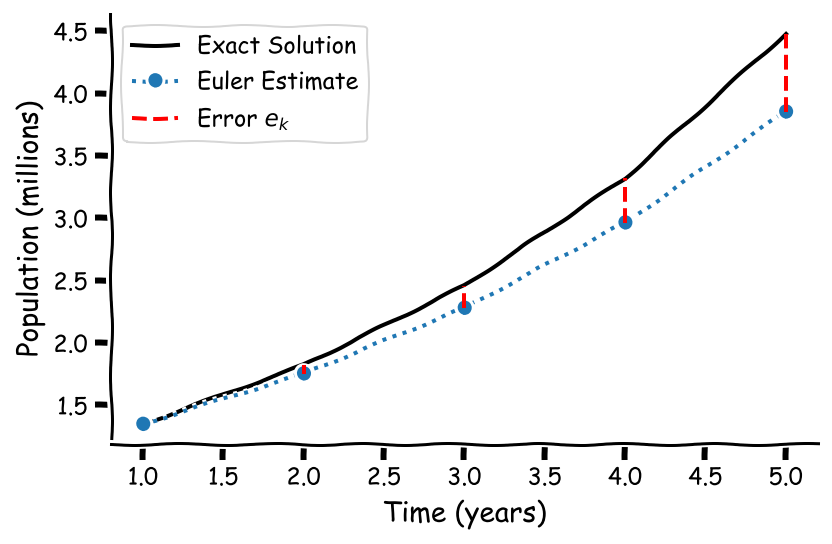
\includegraphics[scale=0.12]{Figures/PreCourse/CFigure7.png}
\end{subbox}

\end{textbox}
%%%%%%%%%%%%%%%%%%%%%%%%%%%%%%%%%%%%%%%%%%%
%%%%%%%%%%%%%%%%%%%%%%%%%%%%%%%%%%%%%%%%%%%
\begin{textbox}{Numerical Method (W0D4T3)}
\begin{subbox}{subbox}{Linear Integrate and Fire }
\scriptsize
The solution of the LIF can be estimated by applying the Euler method to give the difference equation:
\begin{align*}
\color{red}{V[k+1]}=\color{green}{V[k]}+\color{blue}{\Delta t}\big(\frac{-(\color{green}{V[k]}-\color{blue}{E_L}) + \color{blue}{R_m}I[k]}{\color{blue}{\tau_m}}\big),\\
\text{for } k=0\cdots n-1,
\end{align*}

where $\color{green}{V[k]}$ is the estimate of the membrane potential at time point $t[k]$,
 $\color{red}{V[k+1]}$ is the unknown membrane potential at $t[k+1]$, $\color{green}{V[k]} $ is known membrane potential, $\color{blue}{E_L}$, $\color{blue}{R_m}$ and $\color{blue}{\tau_m}$ are known parameters, $\color{blue}{\Delta t}$ is a chosen time-step and  $I(t_k)$ is a function for an external input current.
 
\centering
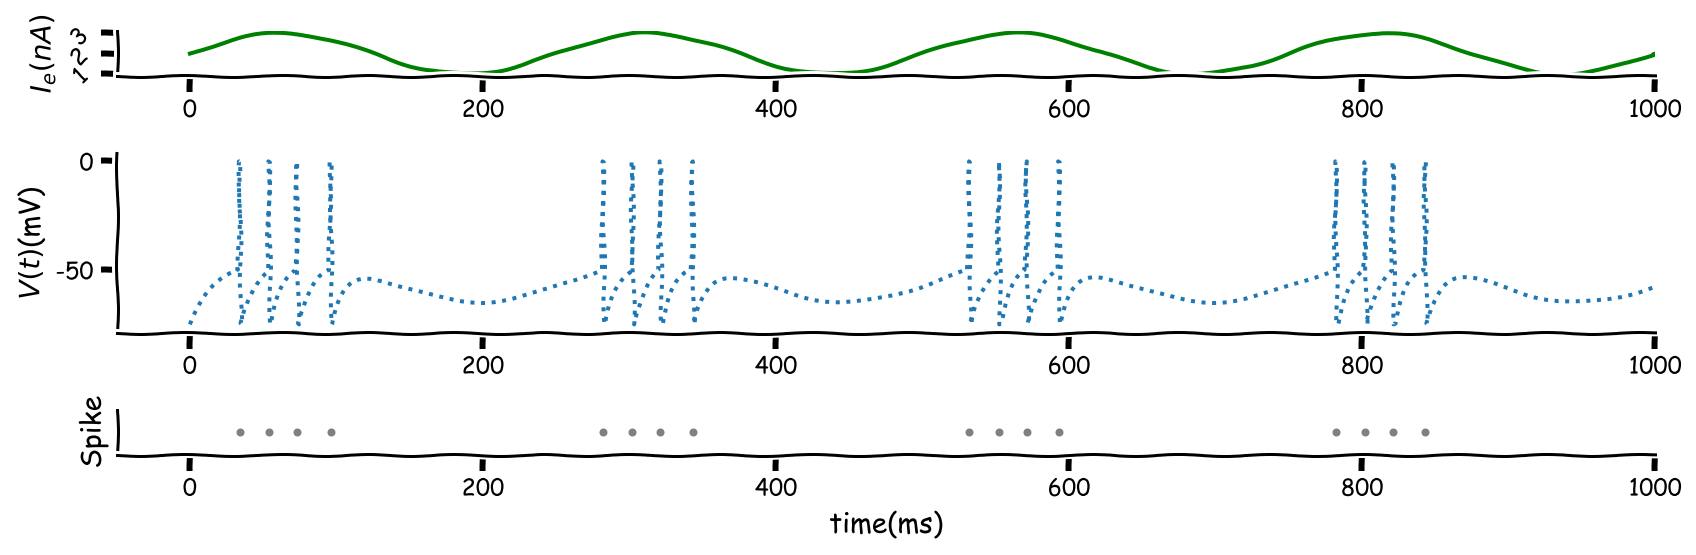
\includegraphics[scale=0.1]{Figures/PreCourse/CFigure8.png}
\end{subbox}

\begin{subbox}{subbox}{Systems of Differential Equations}
\scriptsize
We now model a collection of neurons using a differential equation which describes the firing rate of a population of neurons. 
We will model the firing rate $r$ of two types of populations of neurons which interact, the excitation population firing rate $r_E$ and inhibition population firing rate $r_I$.
 The two coupled differential equations with weights $w$ are:
\begin{align}
\tau_E \frac{dr_E}{dt} &=w_{EE}r_E +w_{EI}r_I, \\
\tau_I \frac{dr_I}{dt} &=w_{IE}r_E +w_{II}r_I ,
\end{align}

The solutions can be approximated using the Euler method such that the equations become:
\begin{align*}
\color{red}{r_E[k+1]}&=\color{green}{r_E[k]}+\color{blue}{\Delta t}\big(\frac{\color{blue}{w_{EE}}\color{green}{r_E[k]}+\color{blue}{w_{EI}}\color{green}{r_I[k]}}{\color{blue}{\tau_E}}\big),\\
\color{red}{r_I[k+1]}&=\color{green}{r_I[k]}+\color{blue}{\Delta t}\big(\frac{\color{blue}{w_{II}}\color{green}{r_I[k]}+\color{blue}{w_{IE}}\color{green}{r_E[k]}}{\color{blue}{\tau_I}}\big),\\
&\text{ for } k=0, \cdots n-1,
\end{align*}
where $r_E[k]$ and $r_I[k]$ are the numerical estimates of the firing rate of the excitation population $r_E(t_k)$ and inhibition population $r_I(t_K)$ and $\Delta t$ is the time-step.

\centering
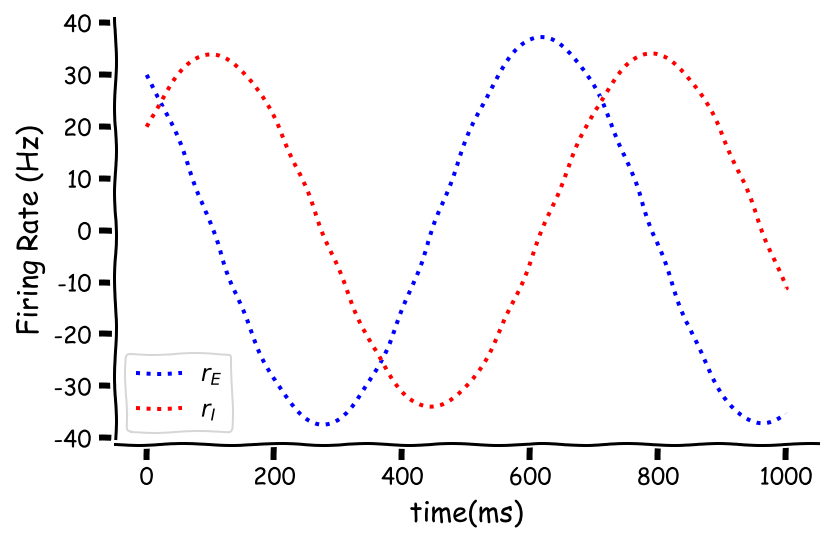
\includegraphics[scale=0.1]{Figures/PreCourse/CFigure9.png}
\end{subbox}
\end{textbox}

\end{multicols}